\documentclass{article}

\usepackage{amssymb}
\usepackage{hyperref}
\usepackage{mathtools}

\title{Automaten en Berekenbaarheid \\ Oplossingen van examenvragen 2016-2017}
\author{Midas Lambrichts}
\date{}

\begin{document}
\maketitle
 
\newpage
\begin{center}
   \textit{This page is intentionally left blank.}
\end{center}
\newpage
\tableofcontents
\newpage
%1
\section{Geef een preciese formulering van het pompend lemma voor reguliere talen en een bewijs ervan. Geef voorbeelden waarbij je laat zien hoe je dat lemma gebruikt om te bewijzen dat een gegeven taal regulier is en om te bewijzen dat een gegeven taal niet regulier is.}
    \subsection{Korte samenvatting van antwoord}    
        Bewijs: neem $d$ meer dan aantal toestanden, dus in string 1 toestand meerdere keren.
    \subsection{Antwoord}
        Te vinden p. 43, Hoofdstuk 2.14.
        \subsubsection{Pompend lemma voor reguliere talen definite:}
        Voor een reguliere taal $L$ bestaat een pomplengte $d$, zodanig dat als $s \epsilon L$ en $\vert s \vert \geq d$, dan bestaat er een verdeling van $s$ in stukken $x$, $y$ en $z$ zodanig dat $s = xyz$ en
        \begin{enumerate}
            \item $\forall i \geq 0: xy^iz \epsilon L$
            \item $\vert y \vert > 0$
            \item $\vert xy \vert \leq d$
        \end{enumerate}
        \subsubsection{Bewijs:}
        Neem een DFA die $L$ bepaalt. Neem $d = \#Q + 1$.
        Neem een willekeurige $s = a_1a_2...a_n$ met $n \geq d$. Beschouw de accepterende sequentie van toestanden ($q_s = q_1, q_2...q_f $) voor $s$; die heeft lengte strikt groter dan $d$, dus zijn er bij de eerste $d$ zeker twee toestanden gelijk (omdat er maar $d - 1$ toestanden zijn). Stel dat $q_i$ en $q_j$ gelijk zijn met $i < j \leq d$ dan nemen we $x = a_1a_2...a_i$ en $y = a_{i+1}...a_j$ en $z$ de rest van de string. Alles volgt nu direct. 

        \subsubsection{Voorbeelden}
            \begin{description}
                \item[Bewijzen dat een taal regulier is:] \hfill  \\
                        Het is niet mogelijk om met het pompend lemma te bewijzen dat een taal regulier is.

                \item[Bewijzen dat een taal niet regulier is:] \hfill \\
                        Neem als taal $\{a^nb^n \vert\  n\ \epsilon\ \mathbb{N} \}$. Stel, de pomplengte is $d$. Neem de string $a^db^d$. Voor iedere opdeling geldt dan dat er meer $a$'s dan $b$'s zullen zijn, omdat $\vert xy \vert \leq d$, dus zal $xy$ altijd uit $a$'s bestaan. Door te pompen zullen er dus meer of minder $a$'s bijkomen, maar geen $b$'s.
            \end{description}

\newpage
%2
\section{Geef een preciese formulering van het pompend lemma voor context-vrije talen en een bewijs ervan. Geef voorbeelden waarbij je laat zien hoe je dat lemma gebruikt om te bewijzen dat een gegeven taal context-vrij is en om te bewijzen dat een gegeven taal niet context-vrij is.}
    \subsection{Korte samenvatting van antwoord}

    \subsection{Antwoord}
        Te vinden op p.72, Hoofdstuk 2.22.
        \subsubsection{Pompend lemma voor CFL definite:}
            Voor een contextvrije taal $L$ bestaat een getal $p$ (de pomplengte) zodanigdat elke string $s$ van $L$ met lengte minstens $p$ kan opgedeeld worden in 5 stukken $u,v,x,y$ en $z$ uit $\sum^*$ zodanig dat $s = uvxyz$ geldt:

            \begin{enumerate}
                \item $\forall i \geq 0: uv^ixy^iz \epsilon L$
                \item $\vert vy \vert > 0$
                \item $\vert vxy \vert \leq p$
            \end{enumerate}

        \subsubsection{Bewijs}
            We gebruiken weer het duivenhokprincipe, maar nu op de parsetree voor lang genoege strings. Neem eerst een CFG in Chomsky normaalvorm voor $L$: dat werkt iets gemakkelijker, want elke regel heeft nu ofwel twee ofwel nul niet-terminalen aan de rechterkant. Laat het aantal niet-eindsymbolen in de CFG n zijn. Voor een string s uit L bestaat er een parse tree. Als je van die boom de onderste takken wegsnoeit hou je een volledige binaire boom over want de grammatica staat in Chomsky normaalvorm. Die boom heeft hoogte minstens gelijk aan $log_2\vert s \vert)$. Het langste enkelvoudig pad van de wortel van die boom bevat dus minstens $log_2\vert s \vert) + 1$ knopen en als we $s$ lang genoeg kiezen, dan is $log_2\vert s \vert) + 1$ groter dan $n$ en bijgevolg moet er op dat langste pad minstens een niet-eindsymbool, zeg $X$, herhaald worden. Neem de laagste $X$ (noteren we door $X_2$) en zijn dichtste herhaling ($X_1$) op dat pad - $X$ is zeker verschillend van het startsymbool (waarom?). We kunnen nu uit die parse tree een afeiding construeren waarvan we enkel wat tussenstappen laten zien: \\
            $S \Rightarrow^* uX_2z  \Rightarrow^* uvX_1yz  \Rightarrow^* uvxyz$ (a) \\
            In die afeiding zijn $u,v,x,y,z$ strings uit $\sum^*$ en bovendien zijn v en y niet tegelijkertijd leeg, want dan zou men uit X zichzelf kunnen afeiden en dat kan niet wegens de vorm van de grammatica. Vermits (a) een geldige afeiding is, is \\
            $S  \Rightarrow^* uX_2z  \Rightarrow^* uxz$\\
            dat ook en ook \\
            $S  \Rightarrow^* uXz  \Rightarrow^* uvXyz  \Rightarrow^* uvvxyyz$ \\
            is er eentje en ... We hebben dus al (1) en (2) van de opgave van de stelling, als we strings nemen die langer zijn dan $2^{(n-1)}$: dat wordt onze pomplengte p. We besluiten nu ook (3): $vxy$ wordt afgeleid vanuit $X$ met een parse tree die kleiner is dan $n$, dus hoogstens $2^{(n-1)}$ bladeren heeft en die corresponderen juist met $vxy$.

        \subsubsection{Voorbeelden}
            \begin{description}
                \item[Bewijzen dat een taal context-vrij is:] \hfill  \\
                        Het is niet mogelijk om met het pompend lemma te bewijzen dat een taal context-vrij is.

                \item[Bewijzen dat een taal niet context-vrij is:] \hfill \\
                        Neem als taal $\{a^nb^nc^n \vert\  n\ \epsilon\ \mathbb{N} \}$. Stel, de pomplengte is $d$. Er zijn nu 2 mogelijkheden, oftwel bestaan $v$ en $y$ uit 1 symbool, waardoor bij het pompen het aantal symbolen niet meer gelijk is, oftewel bestaat het uit meerdere symbolen, waardoor pompen zorgt voor een verkeerde volgorde.
            \end{description}

\newpage
%3
\section{Beschrijf in detail de transformatie van een niet-deterministische eindige toestandsautomaat naar een equivalente deterministische eindige toestandsautomaat. Beschrijf de notie van ``equivalentie van automaten" in deze context en argumenteer waarom de transformatie ``correct" is. Bespreek de uitspraak ``deze transformatie is [niet] deterministisch". (kies zelf of je die ``niet" wil houden of niet)}
    \subsection{Korte samenvatting antwoord}

    \subsection{Antwoord}
            Te vinden p.27, Hoofdstuk 2.11.
            \subsubsection{Transformatie NFA $rightarrow$ DFA}
                \textbf{Gegeven:} een NFA = $(Q_n,\sum, \delta_n,q_{sn}, F_n)$
                \textbf{Gevraagd:} een DFA = $(Q_d,\sum, \delta_d,q_{sd}, F_d)$ zodanig dat $L_{NFA}=L_{DFA}$ \\
                \textbf{Constructie:}
                \begin{description}
                    \item[$Q_d$] = $P(Q_n)$: elke toestand in DFA is verzameling toestanden van NFA.
                    \item[$F_d$] = $\{S \vert\  S\ \epsilon\ Q_d, S \cap F_n \neq \emptyset \}$
                    \item[$\delta_d$] \hfill \\
                        We voeren functie $eb$ (epsilon-bereikbaar) in. Gaat van verzameling toestanden naar verzameling toestanden die met 0, 1 of meer epsilon-bogen bereikbaar zijn vanuit originele verzameling.\\
                        
                        $\delta_d(Q, a) = eb(\delta_n(Q, a))$ voor $Q\ \epsilon\ Q_d$
                    \item[$q_{sd}$] = $eb(q_{sn})$
                \end{description}
            \subsubsection{Equivalentie van automaten}
                We noemen twee automaten $FA_1$ en $FA_2$ equivalent als ze dezelfde taal bepalen.

                De transformatie van een NFA naar een DFA is correct omdat de resulterende DFA de uitvoering van de NFA simuleert. Bij het uitvoeren van een DFA voor een gegeven string kunnen we telkens maar in ´e´en toestand belanden, bij een NFA is dat niet het geval. De transformatie die we toepassen stelt ons in staat om voor elk symbool van een string te bepalen in welke toestand of combinatie van toestanden een NFA zich zal bevinden. Indien ´e´en van die toestanden een eindtoestand is, kan de NFA de string op dat punt ook accepteren. Die constructie zelf is een DFA, omdat we nu voor elk pad door de automaat een deterministisch pad naar combinaties van toestanden hebben bepaald.


            \subsubsection{Deze transformatie is [niet] deterministisch}
                De transformatie is deterministisch omdat de resulterende DFA altijd hetzelfde is voor een bepaalde NFA.
                

\newpage
%4
\section{Beschrijf in detail de transformatie van een deterministische eindige toestandsautomaat naar een equivalente deterministische eindige toestandsautomaat met een minimaal aantal toestanden. Beschrijf de notie van ``equivalentie van automaten" in deze context en argumenteer waarom er geen kleinere equivalente deterministische eindige toestandsautomaat bestaat. Kan een kleinere equivalente niet-deterministische eindige toestandsautomaat bestaan ?}
    \subsection{Korte samenvatting antwoord}

    \subsection{Antwoord}
        \subsubsection{Tranformatie $DFA \rightarrow DFA_{min}$}
            Als we een $DFA(Q,\sum,\delta,q_s,F)$ hebben, construeren we $DFA_{min}(\tilde{Q}, \sum, \tilde{\delta}, \tilde{q_s}, \tilde{F})$ waarbij:
            \begin{itemize}
                \item $\tilde{Q} = {Q_1, Q_2,...}$ waarbij $Q_i$ verkregen wordt door het algoritme om f-gelijke toestanden samen te nemen.
                \item $\tilde{\delta}(Q_i, a) = Q_j$ waarbij $Q_j$ verkregen wordt door: neem een $q \epsilon Q_i$ en neem dan de $Q_j$ zodanig dat $\delta(q,a) = Q_j$
                \item $\tilde{q_s}$ is de $Q_i$ waarvoor geldt $q_s \epsilon Q_i$
                \item $\tilde{F}$ is de verzameling van $Q_i$ waarvoor geldt $Q_i \cap F \neq \emptyset$ 
            \end{itemize}

            Het algoritme voor f-gelijke toestanden te bepalen is kort samengevat als volgt: Stel een graaf $V$ op met als knopen de toestanden. Trek een boog tussen ieder paar toestanden waarvan er juist 1 een eindtoestand is. Ga nu voor ieder paar toestanden dat nog niet verbonden is na of er een $a$ bestaat zodanig dat $(\delta(q,a), \delta(p,a)) \epsilon V$ (in woorden, waarvan een overgang zorgt dat je in het verbonden deel van de graaf komt). Neem nu het complement van de graaf. De verbonden toestanden zijn f-gelijk.

        \subsubsection{Kleinere DFA?}
             Stel $DFA_1$ ($Q_1$, $\Sigma$, $\delta_1$, $q_s$, $F_1$) met $Q_1 = \{q_s,q_1,q_2,...,q_n\}$ is een machine zonder onbereikbare toestanden waarvan elk paar toestanden f-verschillend zijn. Stel dat $DFA_2$ ($Q_2$, $\Sigma$, $\delta_2$, $p_s$, $F_2$) een DFA is met minder toestanden dan $DFA_1$.

            \begin{itemize}
                \item Elke toestand in $DFA_1$ is bereikbaar, dus er bestaan strings $s_i$ met $i=1...n$ zodanig dat $\delta^*_1(q_s,s_i)=q_i$.
                \item $DFA_2$ heeft minder toestanden dan $DFA_1$, dus er is een $i$ en $j$ met $i \neq j$, zodanig dat er strings $s_i$ en $s_j$ zijn waarvoor $DFA_2$ meerdere keren in dezelfde toestand komen, dus $\delta^*_2(p_s,s_i)=\delta^*_2(p_s,s_j)$.
                \item $q_i$ en $q_j$ zijn f-verschillend, dus er bestaat een string $v$ zodanig dat $\delta^*_1(q_i,v) \epsilon F_1 \and \delta^*_1(q_j,v) \notin F_1$ of omgekeerd. Bij gevolg geldt ook $\delta^*_1(q_s,s_iv) \epsilon F_1 \and \delta^*_1(q_s,q_jv) \notin F_1$ of omgekeerd. We zeggen dat $DFA_1$ van $s_iv$ en $s_jv$ just \'e\'en string accepteert.
            \end{itemize}
            
            We kunnen nu aantonen dat $\delta^*_2(p_s,s_iv) = \delta^*_2(\delta^*_2(p_s,s_i),v) = \delta^*_2(\delta^*_2(p_s,s_j),v) = \delta^*_2(p_s,s_jv)$, hetgeen betekent dat $DFA_2$ ofwel beide strings $s_iv$ en $s_jv$ accepteert, ofwel beide verwerpt.
            
            Dus $DFA_1$ en $DFA_2$ kunnen niet dezelfde taal bepalen.

        \subsubsection{Kleinere NFA?}
            Het is mogelijk dat er een kleinere NFA bestaat, omdat de DFA restricties heeft omtrent

\newpage
%5
\section{Bewijs dat een eindige toestandsautomaat altijd een taal herkent die door een reguliere expressie wordt beschreven. Doe dat door een eindige toestandsautomaat te transformeren naar een gegeneraliseerde niet-deterministische eindige toestandsautomaat met slechts 2 toestanden.}
    \subsection{Korte samenvatting antwoord}

    \subsection{Antwoord}
        \subsubsection{GNFA}
            \begin{enumerate}
                \item Maak van de NFA een GNFA: Voeg een nieuwe starttoestand en zet een $\epsilon$-boog van de nieuwe naar de oude starttoestand. Maak op dezelfde manier een nieuwe eindtoestand aan.

                Teken de ontbrekende bogen met een $\emptyset$-boog.

                Als er tussen 2 toestanden parallel gerichte bogen zijn neem ze dan samen met de unie van hun labels ($a\vert b$)

                \item Reduceer de GNFA:
                \begin{itemize}
                    \item Kies een willekeurige toestand $X$, verschillend van start en eindtoestand. Doe voor alle koppels $A$ $B$:
                    \begin{figure}[h!]
                        \centering
                        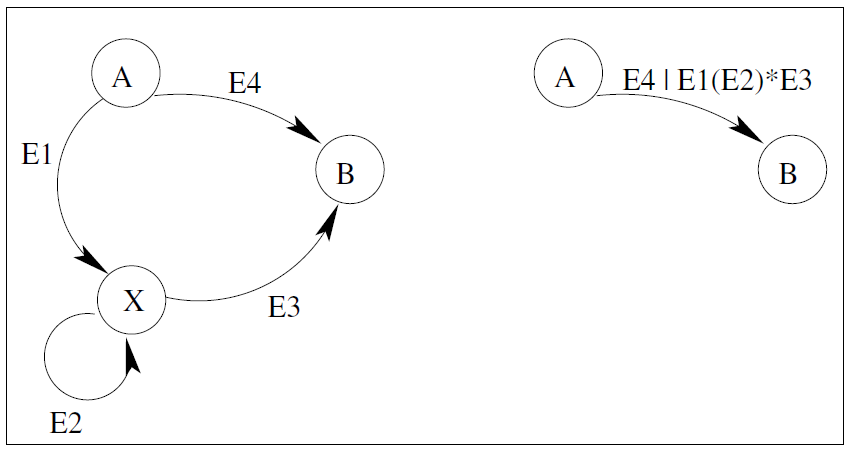
\includegraphics[width=0.8\textwidth]{assets/GNFA-reductie.PNG}
                    \end{figure}

                    Als alle koppels afgelopen zijn, verwijder toestand $X$. Herhaal dit proces tot er geen $X$'en meer gevonden worden.
                \end{itemize}
                \item Uiteindelijk zijn er nog enkel de start en eindtoestand over, op de boog ertussen staat de RE voor de taal die de DFA bepaalde.
            \end{enumerate}

            Bewijzen dat dit correct is gebeurd door te bewijzen dat $GNFA_{voor}$ en $GNFA_{na}$ dezelfde strings accepteren. Dus dat als iets door $GNFA_{voor}$ wordt aanvaard, dan ook door $GNFA_{na}$ en omgekeerd.
\newpage
%6
\section{Bespreek unie, doorsnede, complement, concatenatie van reguliere talen, van contextvrije talen en van niet-contextvrije talen: zijn die operaties inwendig ? Geef voldoende detail in je argumentatie, eventueel voorbeelden indien nuttig.}
    \subsection{Korte samenvatting antwoord}

    \subsection{Antwoord}
        Te vinden op: \url{http://infolab.stanford.edu/~ullman/ialc/spr10/slides/rs2.pdf}
        \subsubsection{Reguliere Talen}
            \begin{description}
                \item[Unie:] Gesloten: $L_1 \cup L_2 = RE_1|RE_2$
                \item[Doorsnede:] Gesloten: Neem het product van de DFA's en neem als eindtoestand de toestanden die in $DFA_1$ en $DFA_2$ eindtoestanden waren.
                \item[Complement:] Gesloten: Het verschil is gesloten (Neem product DFA's en neem als eindtoestand de toestanden die in $DFA_1$ eindtoestand waren, maar niet in $DFA_2$), en complement is eigenlijk $\sum^* - L_1$, wat dus het verschil is tussen 2 Reguliere Talen, wat dus terug regulier is.
                \item[Concatenatie:] Gesloten: $L_1  L_2 = RE_1RE_2$
            \end{description}
        \subsubsection{Contextvrije Talen}
            \begin{description}
                \item[Unie:] Gesloten: Construeer een nieuwe CFG die alle regels van de twee CFG's heeft, en de startregels: $S \rightarrow S_1$ en  $S \rightarrow S_2$
                \item[Doorsnede:] Niet gesloten: neem als voorbeeld $L_1 = \{a^i b^i c^j \vert  i,j \geq 0\}$ en $L_2 = \{a^i b^j c^j \vert  i,j \geq 0\}$, de doorsnede hiervan is $\{a^i b^i c^i  \vert  i \geq 0\}$, wat niet context-vrij is.
                \item[Complement:] Niet gesloten: $A \cap B = \overline{\overline{A} \cup \overline{B}}$ (Als iets gesloten is onder Unie, maar niet onder Doorsnede is het zowiezo niet gesloten onder Complement)
                \item[Concatenatie:] Gesloten: Construeer een nieuwe CFG die alle regels van de twee CFG's heeft, en de startregel: $S \rightarrow S_1S_2$
            \end{description}
        \subsubsection{Niet-contextvrije Talen}
            \begin{description}
                \item[Unie:] \textit{No idea}
                \item[Doorsnede:] Niet gesloten: Neem als voorbeelden $L_1 = \{a^i b^i c^i  \vert  i \geq 0\}$ en $L_2 = \{a^i c^i b^i  \vert  i \geq 0\}$. De doorsnede hiervan is $L_1 \cap L_2 = \{\epsilon\}$ (want enkel voor $i=0$ bepalen beide talen dezelfde string). Dit is een reguliere (en bijgevolg contextvrije) taal.
                \item[Complement:] Niet gesloten: Aangezien het complement van een Contextvrije Taal niet gesloten is, is het complement van een Niet-contextvrije Taal ook niet gesloten.
                \item[Concatenatie:] Niet gesloten: Als een deel van een string niet context vrij is, dan is een concatenatie met een andere string ook zowiezo niet context vrij. (\textit{Denk ik toch})
            \end{description}

\newpage
%7
\section{Definieer de Chomsky Normaal Vorm voor CFGs. Geef de opeenvolgende stappen in het algoritme om een CFG naar een equivalente Chomsky NF te transformeren. Beschrijf de notie van ``equivalentie van grammaticas" in deze context en argumenteer waarom de transformatie ``correct" is. Waarvoor is de Chomsky Normaal Vorm nuttig ?}
    \subsection{Korte samenvatting antwoord}
        
    \subsection{Antwoord}
        \subsubsection{CNF}
            Chomsky Normaal Vorm heeft regels die uit drie vormen mogen bestaan:
            \begin{itemize}
                \item $S \rightarrow \epsilon$
                \item $X \rightarrow AB$
                \item $X \rightarrow \alpha$
            \end{itemize}
            $\alpha$ is een eindsymbool, $X$, $A$, $B$ en $S$ zijn niet-eindsymbolen, en $S$ is het startsymbool.
        \subsubsection{CFG naar CNF}
            \begin{enumerate}
                \item Als $S$ het startsymbool is in de grammatica, vervang het dan overal door een nieuw niet-eindsymbool (bijvoorbeeld $X$) en voeg de regel $S \rightarrow X$ toe.
                \item Als er een regel in de vorm $A \rightarrow \epsilon$ bestaat, voeg dan voor iedere regel $B \rightarrow \beta$ waar $A$ in voorkomt een nieuwe regel toe $B \rightarrow \gamma$ waar $A$ is in weggelaten en verwijder dan $A \rightarrow \epsilon$ (tenzij $A=S$. Blijf dit toen totdat er geen regels meer zijn van de vorm $A \rightarrow \epsilon$.
                \item Als er regels bestaan in de vorm $A \rightarrow B$ en $B \rightarrow \gamma$, voeg dan de regel $A \rightarrow \gamma$ toe en verwijder $B \rightarrow \gamma$
                \item Vervang in iedere regel met meer dan 2 symbolen iedere terminal door een nieuwe niet-terminal $A_a$ en voeg $A_a \rightarrow a$ toe.
                \item Regels van de vorm $A \rightarrow X_1X_2...X_n$ (met $ n > 2$ ) vervang je door $A \rightarrow X_1Y_1$,$Y_1 \rightarrow X_2Y2$,...
            \end{enumerate}
        \subsubsection{Nut}
            Het is gemakkelijk in te zien dat de taal de lege string bepaalt of niet. Bovendien heeft iedere afleiding van een string met van lengte $n > 0$ lengte $2n -1$.


\newpage
%8
\section{Leg uit wat een pushdown automaat is en hoe die werkt. Laat de constructie zien (in het algemeen) van een pushdown automaat die een gegeven contextvrije taal aanvaardt. Argumenteer de correctheid.}
    \subsection{Korte samenvatting antwoord}

    \subsection{Antwoord}
        \subsubsection{PDA}
            Een Push-Down Automaat is een 6-tal $(Q,\sum , \Gamma ,\delta , q_s, F)$, waarbij:
            \begin{itemize}
                \item $Q$ is een eindige verzameling toestanden.
                \item $\sum$ is een eindig inputalfabet
                \item $\Gamma$ is een eindig stapelalfabet
                \item $\delta$ is een overgangsfunctie met signatuur $Q \times \sum_{\epsilon} \times \Gamma_\epsilon \rightarrow P(Q \times \Gamma_\epsilon)$
                \item $q_s$ is de starttoestand
                \item $F \subseteq Q$ is een verzameling eindtoestanden.
            \end{itemize}

        \subsubsection{CFG $\rightarrow$ PDA}
            \begin{itemize}
                \item er zijn slechts 3 toestanden: de begintoestand $q_s$, de eindtoestand $q_f$ en een hulptoestand $x$.
                \item er is slechts een boog van $q_s$ naar $x$: die kijkt niet naar de string of de stapel, en zet een marker \$ op de stapel en het beginsymbool.
                \item er is slechts een boog van $x$ naar $q_f$ : die consumeert niks van de string en haalt demarker \$ van de stapel.
                \item de andere bogen gaan van $x$ naar $x$; de labels corresponderen met
                \begin{itemize}
                    \item de symbolen uit het invoeralfabet: voor elke $\alpha \epsilon \sum$, is er een boog met label $\alpha, \alpha \rightarrow \epsilon$ die bogen betekenen dus: als de top van de stapel gelijk is aan het eerste symbool van de string, consumeer dan beide.
                    \item de regels van de grammatica: voor elke regel $X \rightarrow \gamma$ is er een label $ \epsilon , X \rightarrow \gamma $ die bogen betekenen dus: als de top van de stapel een niet-eindsymbool $X$ is, vervang het door de rechterkant van een regel in de grammatica waarvan $X$ de linkerkant is; is een rij eind- en niet-eindsymbolen
                \end{itemize}
            \end{itemize}

        \subsubsection{Bewijs correctheid}
            


\newpage
%9
\section{ Leg uit wat een pushdown automaat is en hoe die werkt. Laat de constructie zien (in het algemeen) van een CFG die dezelfde taal genereert als een gegeven pushdown automaat. Argumenteer de correctheid.}
    \subsection{Korte samenvatting antwoord}
        
    \subsection{Antwoord}
        \subsubsection{PDA}
            Een Push-Down Automaat is een 6-tal $(Q,\sum , \Gamma ,\delta , q_s, F)$, waarbij:
            \begin{itemize}
                \item $Q$ is een eindige verzameling toestanden.
                \item $\sum$ is een eindig inputalfabet
                \item $\Gamma$ is een eindig stapelalfabet
                \item $\delta$ is een overgangsfunctie met signatuur $Q \times \sum_{\epsilon} \times \Gamma_\epsilon \rightarrow P(Q \times \Gamma_\epsilon)$
                \item $q_s$ is de starttoestand
                \item $F \subseteq Q$ is een verzameling eindtoestanden.
            \end{itemize}
        \subsubsection{$PDA \rightarrow CFG$}
            We veronderstellen dat de PDA van de volgende vorm is:
            \begin{itemize}
                \item er is slechts een eindtoestand
                \item de stapel wordt leeggemaakt voor we daarin terechtkomen
                \item elke transitie neemt een symbool weg van de stapel, of zet er een op, maar niet beide
            \end{itemize}
            Nu kunnen we een CFG contstrueren:
            \begin{itemize}
                \item $V  = A_{p,q}$ waarbij $ p,q\epsilon Q$
                \item $S = A_{q_s, q_f}$
                \item $R$ bestaat uit drie delen:
                \begin{itemize}
                    \item Regels van de vorm $A_{p,p} \rightarrow \epsilon$ voor elke $p \epsilon Q$
                    \item Regels van de vorm $A_{p,q} \rightarrow A_{p,r}A_{r,q}$ voor alle $p,q,r \epsilon Q$
                    \item Regels van de vorm $A_{p,q} \rightarrow aA_{r,s}b$ waarbij $p,q,r,s \epsilon Q, a,b \epsilon \sum_\epsilon, t \epsilon \Gamma, (r,t) \epsilon \delta(p,a,\epsilon), (q,\epsilon) \epsilon \delta(s,b,t)$
                \end{itemize}
            \end{itemize}

\newpage
%10
\section{Geef de definities van ``een taal wordt beslist door een Turing machine" en van ``een taal wordt herkend door een Turing machine". Bewijs dat er een niet-beslisbare taal bestaat, gebaseerd op een cardinaliteitsargument.}
    \subsection{Korte samenvatting antwoord}

    \subsection{Antwoord}
        \subsubsection{Een taal wordt beslist door een Turing machine}
            De TM stopt altijd, voor strings in de taal in een accepterende toestand, voor strings niet in de taal, in een niet-accepterende toestand.

        \subsubsection{Een taal wordt herkend door een Turing machine}
            De TM stopt voor de strings in de taal in een accepterende toestand. Voor strings die niet in de taal zitten blijft de TM oneindig lopen, of stopt hij in een niet-accepterende toestand.

        \subsubsection{Bewijs niet-beslisbare taal met cardinaliteitsargument}
            Elke TM bepaalt juist 1 taal. Het aantal TM is aftelbaar oneindig. Het aantal talen is niet aftelbaar oneindig. Dus zijn er talen die niet herkenbaar zijn, en bijgevolg talen die niet beslisbaar zijn.


\newpage
%11
\section{Definieer de enumerator machine. Bewijs dat elke herkenbare taal kan ge-enumereerd worden en dat elke taal die door een enumerator wordt ge-enumereerd ook herkenbaar is. Kan elke beslisbare taal ge-enumereerd worden ? Bespreek in deze context de uitspraak ``de verzameling van Turing machines is een herkenbare taal".}
    \subsection{Korte samenvatting antwoord}

    \subsection{Antwoord}
        \subsubsection{Enumerator machine}
            Een enumeratormachine is een TM met als extra's:
            \begin{itemize}
                \item Een enumeratortoestand $q_e$
                \item Een outputband
                \item Een outputmarker
            \end{itemize}
            De $\delta$ heeft als overgangsfunctie: $Q \times \Gamma \rightarrow Q \times \Gamma \times \Gamma_\epsilon \times \{L,R,S\}$ ($\Gamma_\epsilon$ is het symbool dat op de outputband wordt geschreven.)

            De machine loopt zoals normaal, waarbij als er iets op de outputband wordt geschreven, de kop ervan naar rechts opschuift. Als de machine in $q_e$ komt, wordt de outputmarker op de outputband geschreven. De machine wordt dan terug in $q_s$ gezet en begint opnieuw. De outputstrings (gescheiden door de marker) noemen we de taal die door de enumerator bepaald is.

        \subsubsection{Elke ge-enumereerde taal is herkenbaar en elke herkenbare taal is enumereerbaar}
            \begin{itemize}
                \item Geef een string s aan de TM. De TM start de Enu. Telkens de Enu in zijn $q_e$ komt, kijkt TM na of de laatst geproduceerde string op de outputband van de Enu gelijk is aan $s$. Indien ja: TM accepteert. Indien niet, laat de Enu verderrekenen.
                \item Herkenbare taal enumereerbaar (door TM):
                \begin{itemize}
                    \item Maak $TM_{gen}$ die de $n$ eerste strings uit $\sum^*$ op de band zet.
                    \item Maak $TM_{n}$ die op elke string, $n$ stappen van de originele TM uitvoert. Als daarbij een string geaccepteerd wordt, schrijf deze dan op de outputband.
                    \item Maak een $TM_{driver}$ die opeenvolgende $n$ genereert en dan $TM_{gen}$ en $TM_n$ oproept.                
                \end{itemize}
            \end{itemize}

\newpage
%12
\section{Bewijs in detail dat $A_{TM}$ niet beslisbaar is - steun daarbij niet op de stelling van Rice. Zou het helpen als het toegelaten was op de stelling van Rice te steunen. Is $A_{TM}$ herkenbaar?}
    \subsection{Korte samenvatting antwoord}

    \subsection{Antwoord}
        \subsubsection{Bewijs}
            Stel er is een beslisser B voor $A_{TM}$. Dat betekent dat bij input $\langle M,s \rangle$ B accepteert als M bij input $s$ stopt in zijn $q_a$ en verwerpt als M bij input $s$ stopt in zijn $q_r$ of loopt.
            We construeren nu een Contradictie machine C met eigenschap $C(\langle M \rangle) = opposite(B(\langle M,M \rangle ))$ .
            $C(\langle C \rangle) = opposite(B(\langle C,C \rangle ))$, wat zorgt voor een contradictie, dus C kan niet bestaan, dus B kan niet bestaan, dus $A_{TM}$ is niet beslisbaar.

        \subsubsection{Steunen op Rice}
            Nee, want Rice steunt op $A_{TM}$
        \subsubsection{Herkenbaar}
            $A_{TM}$ is wel herkenbaar, laat M gewoon lopen op s en accepteer als M accepteert.

\newpage
%13
\section{Formuleer en bewijs in detail de stelling van Rice. Geef voorbeelden van wanneer ze mag toegepast worden en wanneer niet - met argumentie natuurlijk.}
    \subsection{Korte samenvatting antwoord}
        
    \subsection{Antwoord}
        \subsubsection{Formulatie Rice}
            Voor elke niet-triviale, taal-invariante eigenschap $P$ van Turingmachines geldt dat $Pos_P$ (en ook $Neg_P$ ) niet beslisbaar is.
        \subsubsection{Bewijs}
            Stel dat $M_\emptyset$ die de lege taal bepaalt, een eigenschap $P$ niet heeft. Omdat $P$ niet-triviaal is, moet er een machine $X$ bestaan die de taal $L_X$ bepaalt en de eigenschap $P$ wel heeft.

            Stel dat er een beslisser $B$ bestaan voor $Pos_P$, dan kunnen we een beslisser $A$ voor $A_{TM}$ construeren. Voor een gegeven invoer $\langle M,s \rangle$ construeren we een hulpmachine $H_{M,s}$ waarvoor geldt
            \begin{itemize}
                \item $H_{M,s}$ laat $M$ lopen op $s$.
                \item Als $M$ $s$ accepteert, dan laat $H_{M,s}$ $X$ lopen op een invoer $x$ en accepteert indien $X$ $x$ accepteert.
            \end{itemize}
            
            We kunnen zeggen dat voor $H_{M,s}$ geldt dat het de taal $L_X$ bepaalt indien $M$ $s$ accepteert en de lege taal bepaalt indien $M$ $s$ niet accepteert. Dat wilt zeggen dat $H_{M,s}$ de eigenschap $P$ heeft indien $M$ $s$ accepteert en de eigenschap $P$ niet heeft indien $M$ $s$ niet accepteert.
            
            Bijgevolg kunnen we zeggen dat $A$ een invoer $\langle M,s \rangle$ accepteert als $B$ $H_{M,s}$ accepteert en de invoer verwerpt als $B$ $H_{M,s}$ verwerpt. Dus $A$ is een beslisser voor $A_{TM}$, wat niet mogelijk is. Daarom kan de beslisser $B$ voor $Pos_P$ ook niet bestaan.
            
            We zeggen dat $A_{TM}$ reduceerbaar is naar $Pos_P$.
            
            Als $M_\emptyset$ de eigenschap $P$ wel heeft, kunnen we het bewijs uitvoeren voor $\overline{P}$. Omdat we dan bewijzen dat $Pos_{\overline{P}} = Neg_P$ onbeslisbaar is, weten we dat ook $Pos_P = \overline{Neg_P}$ onbeslisbaar is.

        \subsubsection{Voorbeelden}
            Stel dat we de eigenschap bekijken dat een Turingmachine 5 toestanden heeft. We kunnen dit niet gebruiken want dit is niet taal invariant.

            Als we de eigenschap bekijken of een TM een taal accepteert, kunnen we Rice niet gebruiken want dit is een triviale eigenschap (iedere TM accepteert een taal, al is dit de lege taal).


\newpage
%14
\section{Wat is een orakelmachine. Bespreek de uitspraak: ``de verzameling orakelmachines (voor een gegeven orakel) is strikt krachtiger dan de verzameling van Turing machines". Leg hierbij ook uit wat je bedoelt met ``krachtiger". Kan een verzameling orakelmachines (voor bepaald gegeven orakel) alle talen beslissen?}
    \subsection{Korte samenvatting antwoord}

    \subsection{Antwoord}
        \subsubsection{Orakelmachine}
            Een Orakelmachine is een TM die voor een bepaalde vraag de oplossing aan een orakel kan vragen als subroutine. Het Orakel stopt altijd in een eindig aantal stappen.

        \subsubsection{Strikt krachtiger}
            Met krachtiger bedoelt men dat er meer talen mee beslist kunnen worden. Zo kan een Orakelmachine met een orakel voor $A_{TM}$, $E_{TM}$ beslissen.

        \subsubsection{Alle talen}
            Nee, we gebruiken weer het cardinaliteitsargument:
            Het aantal orakelmachines voor een bepaald orakel is aftelbaar oneindig. Terwijl het aantal talen niet-aftelbaar oneindig is, dus zijn er talen die niet door een Orakelmachine beslist kunnen worden.


\newpage
%15
\section{Formuleer en bespreek de stellingen van Church-Rosser. Geef daarbij hun belang i.v.m. het het baseren van een programmeertaal op lambda-calculus. Geef de relatie met de programmeertaal Haskell.}
    \subsection{Korte samenvatting antwoord}

    \subsection{Antwoord}
        \subsubsection{Church-Rosser I}
            Indien $E_1 \xleftrightarrow[]{*}$, dan bestaat er een Expressie $E$ zodanig dat $E_1 \xrightarrow[]{*} E$ en  $E_2 \xrightarrow[]{*} E$

        \subsubsection{Church-Rosser II}
            Indien $E \xrightarrow[]{x} N$ en $N$ staat in normaalvorm, dan bestaat er een reductierij in normaalorde van $E$ naar $N$.


\newpage
%16
\section{Bespreek de Turing-volledigheid van Hornclauselogica. In dezelfde context: bespreek ``subsets" van Hornclauselogica die al dan niet Turing-volledig zijn. Geef de relatie met (zuivere) Prolog.}
    \subsection{Korte samenvatting antwoord}

    \subsection{Antwoord}
        

%%%%%%%%%%%%%%%%%%%%%%%%%%%%%%%%%%%%%%%%%%%%%%%%%%%%%%%%%%%%%%%%%%%%%%%%%%%%%%%%%%%%%%
%%%%%%%%  _   _                  ____                  _   _                  %%%%%%%%
%%%%%%%% | \ | |                / __ \                | | (_)                 %%%%%%%%
%%%%%%%% |  \| | _____      __ | |  | |_   _  ___  ___| |_ _  ___  _ __  ___  %%%%%%%%
%%%%%%%% | . ` |/ _ \ \ /\ / / | |  | | | | |/ _ \/ __| __| |/ _ \| '_ \/ __| %%%%%%%%
%%%%%%%% | |\  |  __/\ V  V /  | |__| | |_| |  __/\__ \ |_| | (_) | | | \__ \ %%%%%%%%
%%%%%%%% |_| \_|\___| \_/\_/    \___\_\\__,_|\___||___/\__|_|\___/|_| |_|___/ %%%%%%%%
%%%%%%%%                                                                      %%%%%%%%
%%%%%%%%%%%%%%%%%%%%%%%%%%%%%%%%%%%%%%%%%%%%%%%%%%%%%%%%%%%%%%%%%%%%%%%%%%%%%%%%%%%%%%


\newpage
%17
\section{Bespreek (eventueel bewijs) de uitspraak: niet elke context-vrije taal is deterministisch. Leg verband met ambiguiteit.}
    \subsection{Korte samenvatting antwoord}

    \subsection{Antwoord}
        \subsubsection{Deterministisch}
            Determinisme in een context-vrije taal komt neer op dat er een CFG voor bestaat die niet ambigu is. Het kan zijn dat voor een bepaalde taal er een ambigue CFG bestaat, maar als er een equivalente CFG bestaat die niet ambigu is dan is de context-vrije taal bepaalt door die CFG deterministisch. Maar er zijn talen waarvoor de CFG inherent ambigu is, dit wil zeggen dat er geen equivalente CFG bestaat die niet ambigu is. Een voorbeeld van zo een taal waarvoor de CFG inherent ambigu is, is: $\{a^nb^nc^m,a^nb^mc^m \vert n,m \geq 0 \}$.

\newpage
%18
\section{Leg het correspondentieprobleem van Post uit. Laat zien dat welk aspect ervan niet beslisbaar is. Is het herkenbaar ?}
    \subsection{Korte samenvatting antwoord}
        Dominostenen. \\
        Kan vertaald worden naar Turingmaching $\rightarrow$ Halting probleem
    \subsection{Antwoord}
        \subsubsection{Post correspondence problem}
            Je hebt een eindig aantal verschillende dominostenen waarbij er vanboven en vanonder een string op staat (elk type domino kan wel oneindig veel voorkomen). Kan je nu een rij stenen zijdelings aaneenleggen zodat de string die vanboven gevormdt wordt gelijk is aan degene die onderaan gevormd wordt?
        \subsection{Beslisbaar?}
            Het is krachtig genoeg om dezelfde berekeningen te doen die een Turingmachine kan. Het stoppen van een willekeurige Turingmachine kan vertaald worden naar het bestaan van een oplossing voor een bepaald PCP. Hierdoor volgt dus dat PCP onbeslisbaar is, want het $H_{TM}$ is onbeslisbaar. Als we het onbeslisbare in termen van PCP gieten: Zolang men niet tot een oplossing is gekomen, kan er altijd een steen bij worden gelegd die potentieel wel voor een oplossing kan zorgen. Je weet nooit wanneer je kan stoppen met stenen bijleggen om tot een oplossing te komen.

            Net zoals $H_{TM}$ herkenbaar is, is dit probleem ook herkenbaar, men kan stoppen als men een oplossing vindt, maar zolang men geen oplossing heeft gevonden kan men door blijven gaan.

\newpage
%19
\section{Bewijs in detail dat elke context-vrije taal herkenbaar is.}
    
    \subsection{Korte samenvatting antwoord}
        
    \subsection{Antwoord}
        Te vinden op: \url{http://www.radford.edu/~nokie/classes/420/Chap4-1.html}
        \subsubsection{Indien CFG gegeven is:}
            We weten dat $A_{CFG}$ beslisbaar is, we gebruiken dit nu om aan te tonen dat elke context-vrije taal, gegeven door zijn CFG ($G$), beslisbaar is. Stel dat we de beslisser voor $A_{CFG}$ S noemen. We construeren een beslisser B voor de CFL die bij input $w$ het volgende doet:
            \begin{itemize}
                \item Maak de string $\langle G, w \rangle$
                \item Laat S lopen op $\langle G, w \rangle$
                \item Als S accept, acept, anders reject.
            \end{itemize}
            We hebben nu een beslisser B voor de context-vrije taal, dus de context-vrije taal is beslisbaar, en bijgevolg ook herkenbaar.
        \subsubsection{Indien CFG niet gegeven is:}

\newpage
%20
\section{Bewijs in detail dat  $REGULAR_{TM}$ niet beslisbaar is. Is diezelfde taal herkenbaar ? Is $\overline{REGULAR_{TM}}$ beslisbaar of herkenbaar?}
    \subsection{Korte samenvatting antwoord}
        Bewijs: Via $A_{TM}$ Hulpmachine $H_s$ die $0^n1^n$ accepteert en iedere andere string accepteert als $M$ $s$ accepteert.
    \subsection{Antwoord}
        \subsubsection{Bewijs}
            Stel dat Turingmachine $R$ een beslisser is voor $REGULAR_{TM}$. We nemen eerst twee willekeurige symbolen die we aanduiden met 0 en 1, en we maken een beslisser $B$ voor $A_{TM}$ als volgt: bij input $\langle M, s \rangle $ doet $B$:
            \begin{itemize}
                \item construeert een hulpmachine $H_s$ die op input $x$ het volgende doet:
                \begin{itemize}
                    \item als $x$ van de vorm $0^n1^n$ is, accept.
                    \item anders: laat $M$ lopen op $s$; als $M$ $s$ accepteert, dan accept $x$.
                \end{itemize}
                \item Laat $R$ lopen op $\langle H_s \rangle$
                \item als $R$ accepteert, accept, als $R$ reject, reject;
            \end{itemize}
            $H_s$ accepteert ofwel de taal $0^n1^n$ (niet-regulier) ofwel heel $\sum^*$ (regulier). Dus $B$ accepteert $\langle M,s \rangle$ alss $R$ $H_s$ accepteert alss $H_s$ heel $\sum^*$ accepteert alss $M$ $s$ accepteert. Dus $B$ is een beslisser voor $A_{TM}$, wat niet kan, dus $REGULAR_{TM}$ is niet beslisbaar.

        \subsubsection{Herkenbaar?}
            
        \subsubsection{$\overline{REGULAR_{TM}}$ beslisbaar of herkenbaar?}
            $\overline{REGULAR_{TM}}$ is zeker niet beslisbaar aangezien $REGULAR_{TM}$ niet beslisbaar is.




\newpage
%21
\section{Geef het bewijs van de stelling $E_{TM}$ is niet beslisbaar. Bespreek daarna de uitspraken $E_{TM}$ is herkenbaar en $E_{TM}$ is co-herkenbaar. (de $E$ staat voor Empty) Ken je ook alternatieve bewijzen ? Hoe zit het met $E_{CFG}$ ?}
    \subsection{Korte samenvatting antwoord}
        
    \subsection{Antwoord}
        \subsubsection{Bewijs}
            Stel dat $E_{TM}$ beslisbaar is, dan bestaat er een beslisser $E$ voor die taal. Construeer nu een beslisser $B$ voor $A_{TM}$ als volgt: $B$ krijgt als input $\langle M, s \rangle$:
            \begin{itemize}
                \item construeer een machine $M_s$ die als volgt te werk gaat: voor input $w$ doet $M_s$:
                \begin{itemize}
                    \item indien $w \neq s$, reject.
                    \item laat $M$ lopen op $w$ en geef zelfde resultaat.
                \end{itemize}
                \item Laat $E$ lopen op $\langle M_s \rangle$
                \begin{itemize}
                    \item Indien $E$ accept, reject (bepaalde lege taal), als $E$ reject, accept ($M$ accepteerde $s$)
                \end{itemize}
            \end{itemize}
            $B$ is dus een beslisser voor $A_{TM}$, wat niet kan dus kan $E$ niet bestaan en is $E_{TM}$ niet beslisbaar.

        \subsubsection{Herkenbaar/Co-herkenbaar}

        \subsubsection{Alternatieve bewijzen}

        \subsubsection{$E_{CFG}$}
            $E_{CFG}$ is beslisbaar. We beschrijven een algoritme om een CFG om te vormen zodat de beslissing gemakkelijk is:
            \begin{itemize}
                \item Als er een regel $A \rightarrow \alpha$ (met $\alpha$ alleen eindsymbolen), vervang overal aan de rechterkant $A$ door $\alpha$.
                \item Blijf dit doen tot
                \begin{itemize}
                    \item Het startsymbool verwijdert is: reject want string kan afgeleid worden.
                    \item Geen regels meer over: accept.
                \end{itemize}
            \end{itemize}

\newpage
%22
\section{Geef het bewijs van de stelling $EQ_{TM}$ is niet beslisbaar. Kan (een variante van) de stelling van Rice helpen om dit te bewijzen ?}
    \subsection{Korte samenvatting antwoord}

    \subsection{Antwoord}
        \subsubsection{Bewijs}
            We weten al dat $E_{TM}$ niet beslisbaar is, en eigenlijk is dit hier een speciaal geval: het is duidelijk dat als we van twee willekeurige machines kunnen beslissen of ze dezelfde taal genereren, dan moet dat ook kunnen met een willekeurige machine en $M_\emptyset$ (de machine waarvan de taal leeg is). Bijgevolg krijgen we een contradictie door te veronderstellen dat $EQ_{TM}$ beslisbaar is.


\newpage
%23
\section{Bespreek de twee noties van reduceerbaarheid ($A \leq_m B$ en $A \leq_T B$), hun verband en op welke manier die noties kunnen gebruikt worden om aan te tonen dat een taal (on)beslisbaar/herkenbaar is.}
    \subsection{Korte samenvatting antwoord}
        
    \subsection{Antwoord}
        \subsubsection{Reduceerbaarheid}
            \begin{description}
                \item[Many-one reduction] \hfill \\
                        We zeggen dat taal $L_1$ (over $\sum_1$) naar taal $L_2$ (over $\sum_2$) kan gereduceerd worden indien er een afbeelding $f$ met signatuur $\sum_1^* \rightarrow \sum_2^*$ bestaat zodanig dat $f(L_1) \subseteq L_2$ en $f(\overline{L_1}) \subseteq \overline{L_2}$ en zodanig dat $f$ Turing-berekenbaar is.
                        We noteren door $L_1 \leq_m L_2$
                \item[Turingreduceerbaar] \hfill \\
                        Een taal A is Turingreduceerbaar naar taal B, indien A beslisbaar is relatief t.o.v. B, t.t.z. er bestaat een orakelmachine $O^B$ die A beslist. We schrijven A $\leq_T$ B.
            \end{description}
            \begin{itemize}
                \item $\leq_m$ is fijner dan $\leq_T$ ($A \leq_m B \Rightarrow A \leq_T B$)
                \item Als $L_1 \leq_m L_2$ en $L_2$ is herkenbaar/beslisbaar, dan is $L_1$ herkenbaar/beslisbaar
                \item  Als $L_1 \leq_m L_2$ en $L_1$ is niet beslisbaar/herkenbaar, dan is $L_2$ niet beslisbaar/herkenbaar.
            \end{itemize}



\newpage
%24
\section{Geef de opbouw van de primitief recursieve functies, en die van de recursieve functies. Argumenteer waarom al die functies met een Turingmachine kunnen berekend worden, en omgekeerd. Is er een verband tussen de berekenbaarheid van een functie en de grootte van zijn domein en/of bereik?}
    \subsection{Korte samenvatting antwoord}

    \subsection{Antwoord}
        \subsubsection{Opbouw primitief recursieve functies}


\newpage
%25
\section{Geef informeel de definitie van een {\em lineair begrensde automaat} (LBA). Argumenteer dat het aanvaardingsprobleem voor LBA's ($A_{LBA}$) beslisbaar is. Geef de stappen in een bewijs dat $E_{LBA}$ (de verzameling van LBA's die de lege taal bepalen) niet beslisbaar is.}
    \subsection{Korte samenvatting antwoord}

    \subsection{Antwoord}
        \subsubsection{Definitie LBA}
            Een Lineair Begrensde Automaat is een Turingmachine die niet leest of schrijft buiten het deel van de band dat initieel invoer bevat.
        \subsubsection{Bewijs $A_{LBA}$ beslisbaar}
            We kijken naar de conguraties die kunnen voorkomen tijdens de uitvoering van een LBA op een string met lengte $n$. Het aantal toestanden van de LBA noteren we met $q$ en het aantal elementen in het bandalfabet met $b$. Het aantal mogelijke strings die tijdens de uitvoering op de band kunnen staan is begrensd door $b^n$. De leeskop kan onder elk van de symbolen staan terwijl de machine in elk van de toestanden kan zitten. Dat geeft in het totaal maximaal $qnb^n$ conguraties.
            We kunnen nu een beslisser B voor ALBA construeren als volgt: bij input $\langle M, s \rangle$ doet B het volgende:
            \begin{itemize}
                \item Berekent $Max=qnb^n$
                \item simuleert dan $M$ op $s$ voor maximaal $Max$ stappen.
                \item indien ondertussen accept, accept
                \item indien ondertusen reject, reject
                \item indien $M$ nog niet stopte, reject (lus)
            \end{itemize}
        \subsubsection{Bewijs $E_{LBA}$ niet beslisbaar}
            Stel dat we een beslisser $E$ hebben voor $E_{LBA}$. We construeren een beslisser $B$ voor $A_{TM}$ als volgt. Bij input $\langle M, s \rangle $ doet $B$:
            \begin{itemize}
                \item construeer de $LBA$ $A_{M,s}$ die van input kan beslissen of een inputstring een accepterende computation history is voor $M$ op input $s$
                \item laat $E$ los op $\langle A_{M,s} \rangle$: als $E$ aanvaardt, reject; anders accept
            \end{itemize}
            $B$ beslist dus $A_{TM}$, wat niet kan, dus $E_{LBA}$ is niet beslisbaar.



\newpage
%26
\section{Bespreek berekenen door middel van samenwerkende eindige automaten.}
    \subsection{Korte samenvatting antwoord}
        
    \subsection{Antwoord}
        Een voorbeeld hiervan is een cellulaire automaat: Een verzameling identieke eindige toestandsmachines die regelmatig en tegelijk van toestand veranderen. De toestand hangt ook af van de toestand van de buren.

        Een klassiek probleem hiervoor is The Firing Squad Problem. Waarbij een generaal tegen de soldaat naast hem kan praten, en de soldaten in de rij enkel met de soldaten direct naast hun. De vraag is nu hoe we ze allemaal tegelijk kunnen laten vuren? Dit is een vorm van synchronisatieprobleem.

\end{document}